\chapter{Projecto}


\section{Material}
\begin{table}[H]
	{\rowcolors{3}{green!80!yellow!50}{green!70!yellow!40}
		\begin{tabular}{ |p{12cm}|c|p{2cm}|  }
			\hline
			\multicolumn{3}{|c|}{Lista de Material} \\
			\hline
			Peça & Quant & Preço [uni] \\
			\hline
			Fonte de alimetação 12V 1A & 1 & \EUR{3.87} \\
			Conversor DC-DC com voltímetro & 1 & \EUR{7.75} \\
			ET BASE AVR Atmega128 Board & 1 & \EUR{23.92} \\
			Test Input Board  & 1 & \EUR{3.71} \\
			Test Output Board & 1 & \EUR{3.71} \\
			IDC Socket 10 way    & 12 & \EUR{0.31} \\
			IDC Header Straight 10 way    & 12 & \EUR{0.25} \\
			Flatcable    & ? & \EUR{?} \\
			20x4 LCD Module Blue & 1 & \EUR{12.24} \\
			SparkFun Load Cell Amplifier HX711 & 1 & \EUR{13.04}   \\
			50Kg Load Cell & 1 & \EUR{12} \\
			\hline
			 & \textit{total} & \EUR{86.96} \\
			\hline
		\end{tabular}
	}
	\caption{Lista de material}
	\label{material}
\end{table}
Sem contar com as despesas no equipamento para a programação do hardware que em principio só se gasta uma vez, isto é, se não se estragar. No caso do programador da Atmel o \textbf{ICE} pode custar até \EUR{185.55}.\\
\\
É de ter em conta que os preços são \textbf{PVP}, que no caso se for preços comerciais são dez vezes inferior, e se for para produção em grande escala também tem descontos por quantidade.\\
\\
\\


\begin{figure}[H]
	\captionsetup{justification=raggedright,singlelinecheck=false}
	\flushleft
	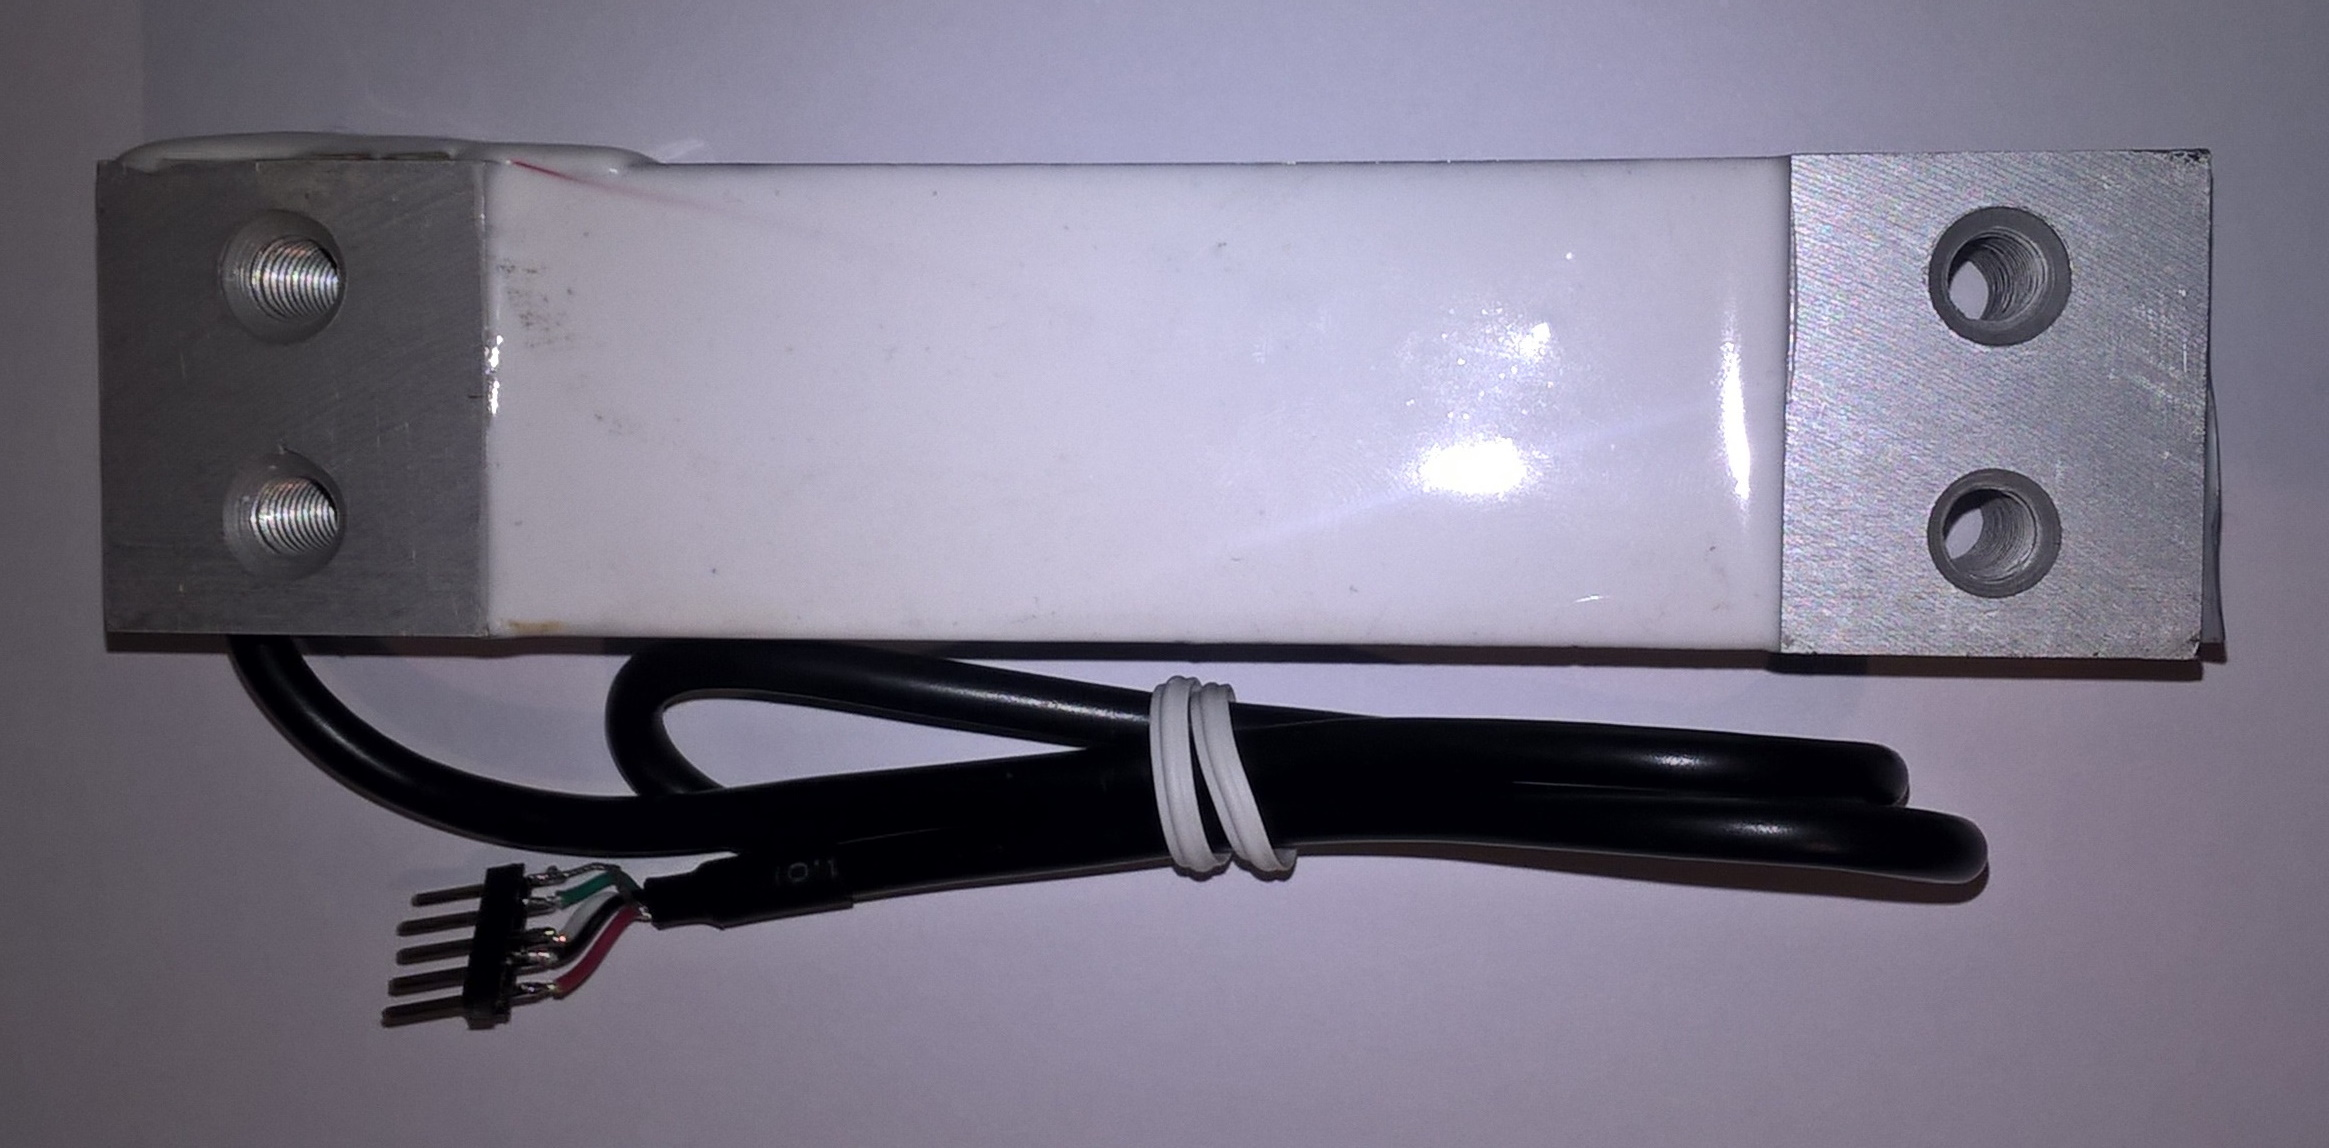
\includegraphics[scale=0.15]{./image/PESTA/material/Load_Cell_1.jpg}
	\caption{Load Cell 50Kg}
	\label{Load_Cell_1}
\end{figure}

\begin{figure}[H]
	\captionsetup{justification=raggedright,singlelinecheck=false}
	\centering
	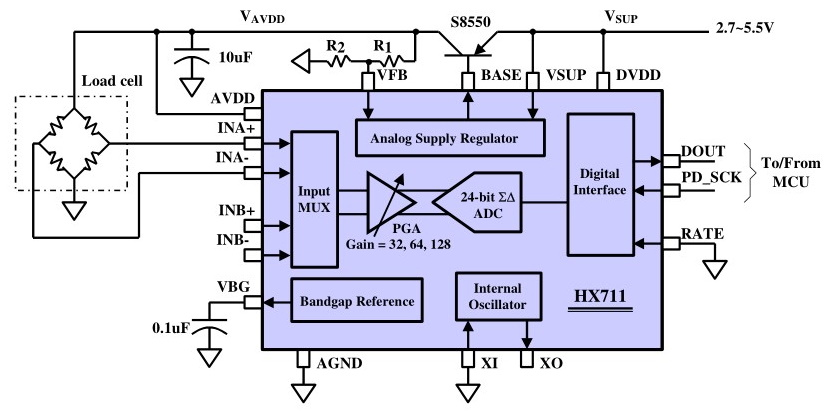
\includegraphics[scale=0.35]{./image/PESTA/schematic/HX711_Schematic_1.jpg}
	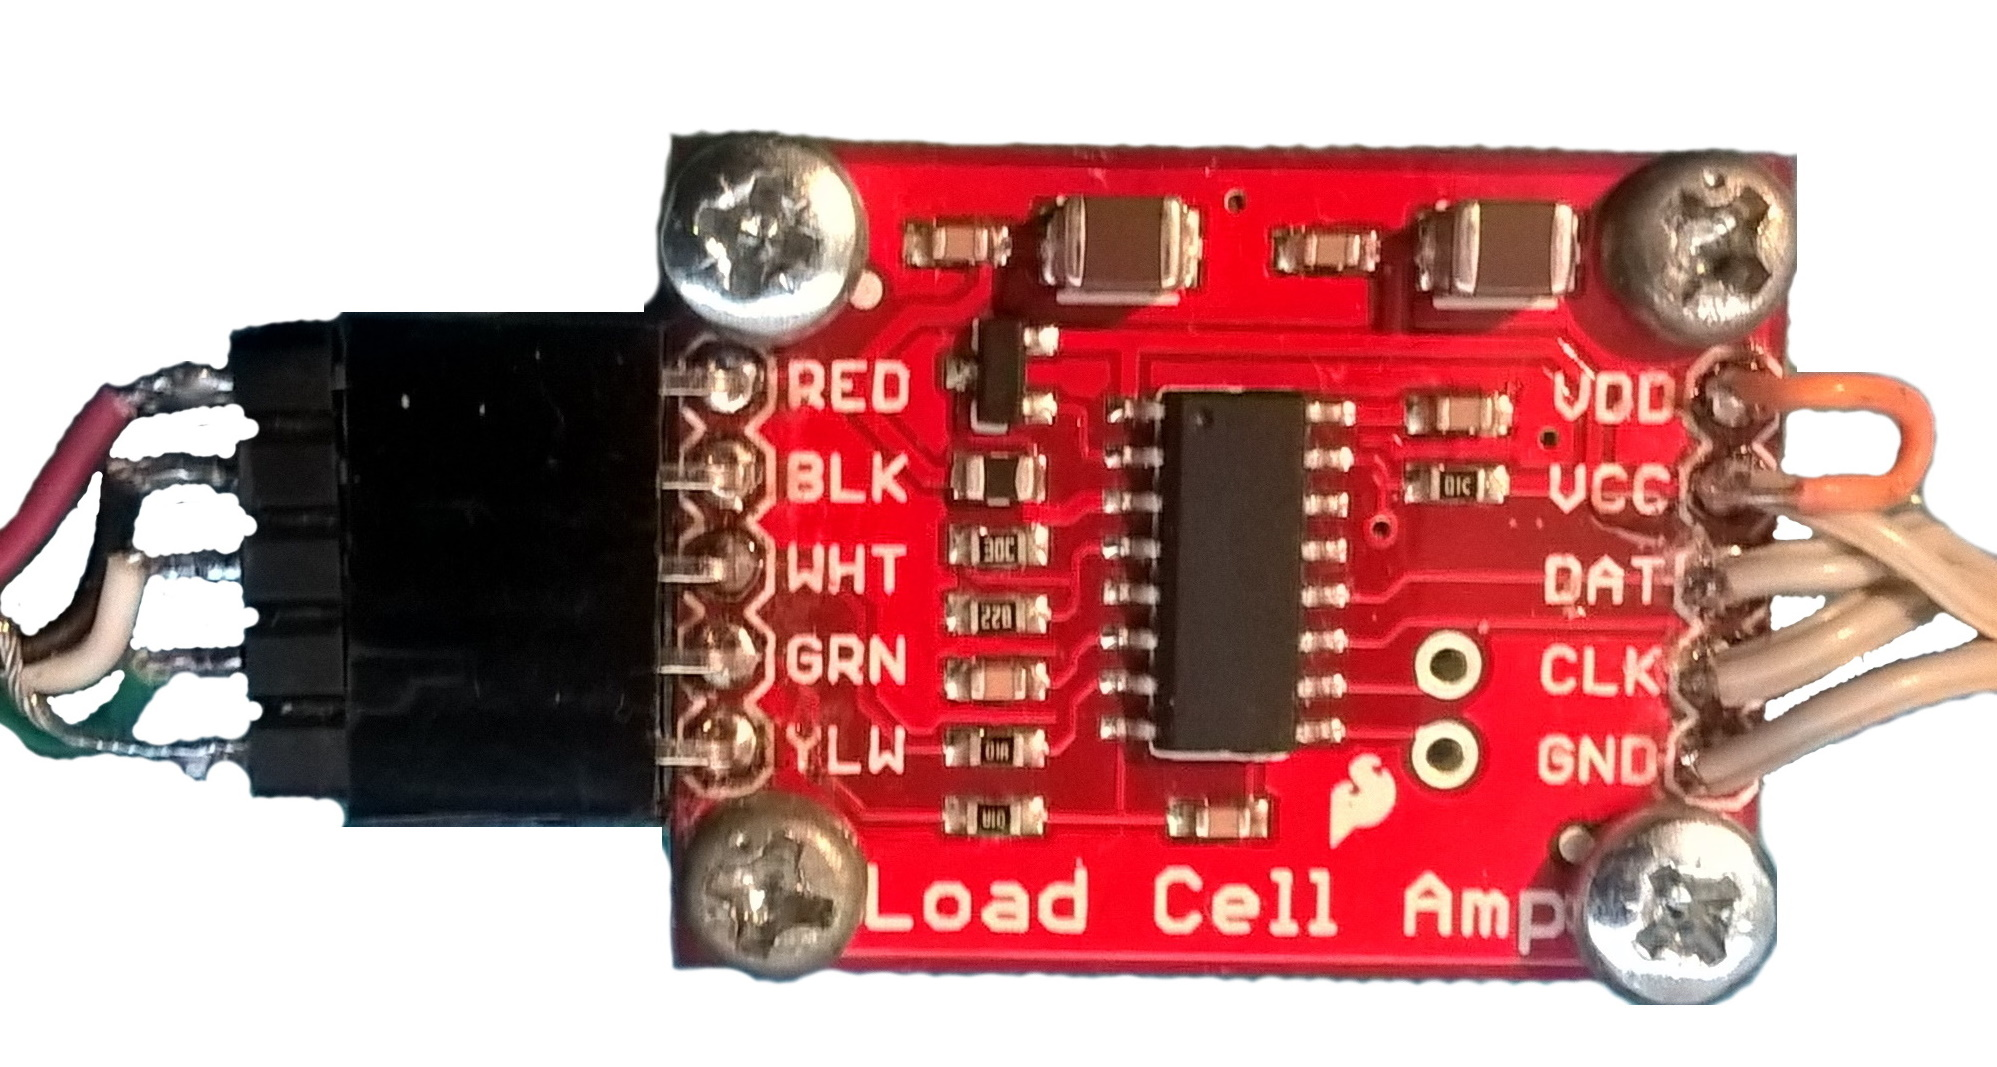
\includegraphics[scale=0.1]{./image/PESTA/material/HX711_board_1.jpg}
	\caption{Load Cell Amplifier [HX711]}
	\label{HX711_Schematic_1}
\end{figure}



